\documentclass[10pt,twocolumn,letterpaper]{article}

\usepackage{cvpr}
\usepackage{times}
\usepackage{epsfig}
\usepackage{graphicx}
\usepackage{amsmath}
\usepackage{amssymb}
\usepackage{url}
\usepackage{subcaption}
\usepackage{float}
\usepackage{array}
\usepackage{balance}

% Include other packages here, before hyperref.

% If you comment hyperref and then uncomment it, you should delete
% egpaper.aux before re-running latex.  (Or just hit 'q' on the first latex
% run, let it finish, and you should be clear).
\usepackage[breaklinks=true,bookmarks=false]{hyperref}

\cvprfinalcopy % *** Uncomment this line for the final submission

\def\cvprPaperID{****} % *** Enter the CVPR Paper ID here
\def\httilde{\mbox{\tt\raisebox{-.5ex}{\symbol{126}}}}

% Pages are numbered in submission mode, and unnumbered in camera-ready
%\ifcvprfinal\pagestyle{empty}\fi
\setcounter{page}{1}
\begin{document}

%%%%%%%%% TITLE
\title{Gaze Estimation for Mobile Security Application in iOS}

\author{Alvin Chou\\
Carnegie Mellon University\\
5000 Forbes Avenue, Pittsburgh, PA 15213\\
{\tt\small alvincho@andrew.cmu.edu}
% For a paper whose authors are all at the same institution,
% omit the following lines up until the closing ``}''.
% Additional authors and addresses can be added with ``\and'',
% just like the second author.
% To save space, use either the email address or home page, not both
}

\maketitle
%\thispagestyle{empty}

%%%%%%%%% ABSTRACT
\begin{abstract}
Security applications in mobile platforms is at the forefront of technology evolution as mobile computing now takes up more internet bandwidth than its alternatives.  Existing security measures for mobile platforms, like passwords, pattern locks, and facial recognition are all valid but breachable measures that are flawed in their own ways.  This paper introduces a novel approach in mobile security by using computer vision to create a gaze estimation protocol in which mobile devices can be unlocked through eye gaze patterns.  In addition, this paper focuses on its application in mobile computing and optimization for real-time performance.   
\end{abstract}

%%%%%%%%% BODY TEXT
\section{Introduction}
Accurate gaze estimation is fast becoming an increasingly important topic in computer vision regarding their practical applications, especially in mobile platforms.  Increasingly, commercial industries are becoming interested gaze estimation technologies, especially in performing marketing studies to promote the right ads at the right locations on a browser or in a store.  However, this technology can be extended to mobile security measure as well, and this paper looks into its application and optimization on a mobile platform for a pattern lock on mobile using gaze estimation.  This paper provides an approach to create gaze estimation using only the monocular camera available on most mobile platforms through image filters and circle hough transforms. It also presents optimization by using a system-on-chip approach to capitalize on the GPU processing and accelerated matrix arithmetic.  This paper also presents various comparisons among different image processing techniques and evaluate each resulting performance based on speed and real-time application.  Finally, the paper presents a threshold system for gaze estimation mapping and how it can be applied in pattern lock technology. 

\section{Background}
Conventional security application in mobile in the form of passcode protection has long been in existence since before smart mobile devices reach the mass market.  In addition, as Android devices become popular, additional security measures in the form of pattern locks has been introduced where users can specify a unique patterns formed by a grid of dots on a touchscreen.  Recently, Apple introduced the idea of fingerprint ID by embedding a biometric sensor in its smartphones.  All of these present certain challenges and flaws specific to the mobile computing platform, however.  The passcode and pattern locks often leave behind visible trails of where the fingers were on the touchscreen, allowing other users to often correctly guess the correct passcode/pattern based on brute-force search given the reduced constraints.  In addition, even though biometric sensors greatly limited accessibility by other users, its difficulty in user interaction and the cost of additional hardware components pose as challenges to its mass adoption.

Recent introductions of facial-based recognition security measures attempt to provide alternatives to conventional approaches.  Intel has since introduced facial recognition security measures that uses facial features of a person as matching criteria.  This approach is problematic in its inability to discern between a real person and a photograph of the same person.  Another approach done by Uchida et al. \cite{3dface} uses passive stereo cameras to create 3D facial recognition technology.  While this is important in passing the photograph test, its impracticality at the present due to the lack of mass adaptation of stereo cameras on mobile devices pose as its limitation. 

In Heyman \cite{heyman}, an approach was proposed using only the monocular camera to train a CANDIDE-3 3D face model and apply Canonical Correlation Analysis \cite{candide}.  This model was able to accurately estimate the gaze direction in three dimensions using a desktop platform with good results.  However, the application was done using a desktop platform without optimization for a mobile setting.

\section{Approach}
In the study, two approaches were considered for facial feature extraction: a CANDIDE-3 model and 2D facial detection.  After the eye features are extracted, the eye image patches are filtered for pupil extraction with circle hough transform.  Finally, given the calculated position of the pupil centroids, a pattern lock app is developed using the estimated gaze movement to threshold and categorize gaze direction sequences.
\subsection{Facial Feature Extraction}
The first attempt in facial feature extraction uses a CANDIDE-3 face modeling library provided by \cite{candide}.  The package, however, only provide cross-platform compilation and lacks mobile optimization capability.  In addition, its APIs are difficult to integrate and its performance is questioned.
\begin{figure}[h]
\begin{center}
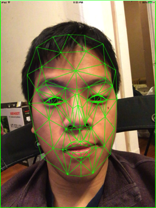
\includegraphics[width=0.4\linewidth]{candide-3.png}
\end{center}
   \caption{3D face modeling using CANDIDE-3 library}
\label{candide}
\end{figure}

The second approach is to utilize the system-on-chip hardware for facial feature detection.  Two methods are used for comparison: OpenCV with Haar Cascade and a GPU-based approach using CoreImage. The OpenCV approach with Haar Cascade detects the position and size of both the face and the eyes.  This approach uses CPU processing and is easy to implement.  On the other hand, the CoreImage library provided by Apple uses a GPU-based detection for face, eyes, and mouth.  The output of this approach returns the size and position of the face, the position of the centers of the eyes, and the position of the mouth. Even though this approach is somewhat more involved in setting up, it is interesting to observe any speed up in performance due to its optimization in GPU.

\subsection{Pupil Extraction}
Given the eye patch images extracted from the facial detection steps, the next step is to extract the location of the pupils in relation to the frame of the eye patch image.  Since it can be inferred that the pupil is the darkest blob of reasonable size in the image, we can extract the pupil by looking for a shape that fits a dark circle well.  The process is done using steps similar to \cite{pupil}:
\begin{enumerate}
\item \textbf{Inversion Filter} to accentuate and differentiate the pupil from the rest of the features.
\item \textbf{Grayscale Filter} to convert BGR color scheme to a single-layered intensity values.
\item \textbf{Threshold Filter} to narrow down possible candidates for pupil based on color intensity.
\item \textbf{Circle Hough Transform} implementation to identify the most probable location of the pupil.
\end{enumerate}

In evaluating performance for mobile applications, two methods of filters will be used and evaluated: OpenCV filters and GPUImage filters.  However, since Circle Hough Transform is only available in the form of OpenCV, the comparison between the performance of OpenCV filters and GPUImage filters does not include the Circle Hough Transform in either case.

After the centroids of the pupil are defined, a smoothing algorithm was used as tracking through a 3-frame moving average algorithm.  The process seeks to strike a balance between stability of the centroid extraction across frames versus the real-time performance of the system.  The final position of the centroid for $t$ is as follows
\begin{equation} \label{eq1}
\begin{split}
x_t & = \frac{x_{extracted,t}+x_{t-1}+x_{t-2}}{3} \\
y_t & = \frac{y_{extracted,t}+y_{t-1}+y_{t-2}}{3} \\
\end{split}
\end{equation}

Even though this results in much less variation and unstable fluctuation of the estimated position, the moving average delays the convergence of the centroid by factoring in past data and instills a sense of "lag" in the overall performance even though the system is achieving real-time performance.

\subsection{Estimated Gaze Pattern Sequence}
After the positions of the pupils are determined, the gaze direction sequence is captured and categorized in relation to the initial positions of the pupils when they are looking directly forward.  The different gaze direction categories are determined as:
\begin{itemize}
\item \textbf{Center}: When both the left and right pupils are within 5 pixels of their original positions.
\item \textbf{Left}: When the left eye is at least 10 pixels away from its centered position in x-direction.
\item \textbf{Right}: When the right eye is at least 10 pixels away from its centered position in the x-direction.
\item \textbf{Up}: When both the left and right eyes are at least 5 pixels above their centered positions in the y-direction.
\item \textbf{Down}: When both the left and right eyes are at least 5 pixels below their centered positions in the y-direction.
\end{itemize}

The system will register the centered direction after the user has looked at the center for the beginning two seconds of the process.  Thereafter, the system will create a sequence of directions whenever the user looks in any direction (left, right, up, down) and returns to the center immediately afterwards.  This sequence of directions is matched to the pre-determined sequence required to unlock the device.  If the pattern does not match, the current registered pattern state is reset.

\section{Results}
\subsection{Facial Feature Detection}
In performing facial feature detection, three approaches are used: CANDIDE-3 face model, OpenCV face detection with Haar Cascade, and CoreImage feature detection.  The approach using CANDIDE-3 model is not successful due to the difficulty in API availability of the library and its cross-platform architecture with a lack of focus on mobile optimization.

In comparison between facial feature extractions using OpenCV versus Apple's CoreImage, it is apparent that CoreImage is 30\% faster than the OpenCV implementation, as shown in Table \ref{table:FPS}.  For the OpenCV implementation, Haar Cascade frontal face and eye detectors are used.  From the study, it is shown that the OpenCV implementation is not able to achieve a real-time performance of 30 FPS on average.  This leads to a significant delay in performance as shown in Figure \ref{compare}.

The CoreImage implementation, however, was able to achieve an average frame rate of 35.68 FPS.  This yields a 30\% improvement in performance over OpenCV, and since it is above the refresh rate of 30 FPS, the CoreImage implementation allows for real-time performance.  The results from Instruments for the comparison is shown in Figure \ref{instruments} and the output comparison is shown in Figure \ref{compare}.
\\

\begin{table}[h]
\begin{center}
\begin{tabular}{|l|c|}
\hline
Method & Average FPS \\
\hline\hline
OpenCV & 27.32 \\
CoreImage & 35.68 \\
\hline
\end{tabular}
\end{center}
\caption{Performance comparison between OpenCV and CoreImage facial feature detection}
\label{table:FPS}
\end{table}

\begin{figure}[h!]
    \centering
    \begin{subfigure}[t]{0.5\linewidth}
        \centering
        \includegraphics[scale=0.06]{opencv}
        \caption{OpenCV face detection with Haar Cascade}
    \end{subfigure}%
    ~ 
    \begin{subfigure}[t]{0.5\linewidth}
        \centering
        \includegraphics[scale=0.06]{coreimage}
        \caption{CoreImage implementation}
    \end{subfigure}
    \caption{Comparison of real-time output between OpenCV and CoreImage}
    \label{compare}
\end{figure}

\begin{figure}[t!]
\centering    
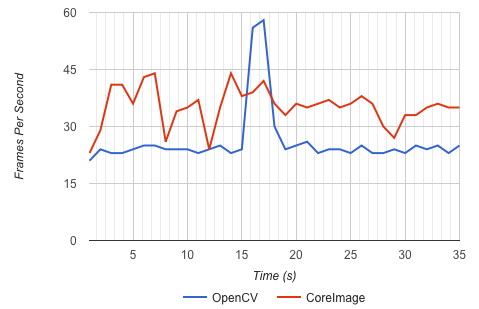
\includegraphics[scale=0.5]{instruments}
\caption{OpenCV vs CoreImage speed for 35 seconds}
\label{instruments}
\end{figure}

\subsection{Pupil Extraction}
Given the extracted images of the left and right eyes via feature detection, pupils are extracted from these image patches using the inversion filter, the grayscale filter, the threshold filter, and finally the circle Hough Transform. Through manual tuning, the best results were achieved using the following parameters:

\begin{enumerate}
\item \textbf{Inversion} - Directly invert all BGR color values
\item \textbf{Grayscale} - Converts inverted image to grayscale
\item \textbf{Threshold} - Threshold the grayscale image at 220.  All intensity values above 220 are kept while all intensity values below 220 are set to 0.
\item \textbf{Circle Hough Transform} - Use a minimum distance of 1/4 the height of the image between circles, an accumulator threshold of 20, and a circle radius between 1/8 of the width of the image to 1/5 of the same width.
\end{enumerate}

\begin{figure}[H]
    \centering
    \begin{subfigure}[t]{0.5\linewidth}
        \centering
        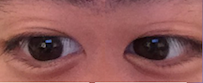
\includegraphics[scale=0.5]{original}
        \caption{Original eye patch images}
    \end{subfigure}%
    ~ 
    \begin{subfigure}[t]{0.5\linewidth}
        \centering
        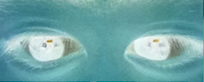
\includegraphics[scale=0.5]{invert}
        \caption{Color inversion}
    \end{subfigure}
    ~ 
    \begin{subfigure}[t]{0.5\linewidth}
        \centering
        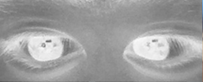
\includegraphics[scale=0.5]{gray}
        \caption{Grayscale}
    \end{subfigure}%
    ~ 
    \begin{subfigure}[t]{0.5\linewidth}
        \centering
        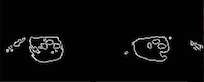
\includegraphics[scale=0.5]{threshold}
        \caption{Threshold}
    \end{subfigure}
    ~ 
    \begin{subfigure}[t]{0.5\linewidth}
        \centering
        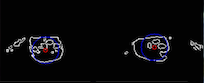
\includegraphics[scale=0.5]{final}
        \caption{Circle Hough Transform}
    \end{subfigure}
    \caption{Pupil extraction process}
    \label{pupil}
\end{figure}

Given a good knowledge of the relationship between the pupil and the eye image, a good result is achieved as shown in Figure \ref{pupil}.  Even though the resulting filtered images are not perfect and can be further refined, a main constraint is that the variability in each test is subject to the environment at each instance.  Different lighting conditions, user's facial characteristics, and camera parameters all impact the resulting filtered image outcome and the tuning parameters required for the image processing to work well.

In comparison between OpenCV filters and GPUImage filters, no significant difference is found, as shown in Table \ref{table:filters}.  An observation made in the case attributes the identical performance of either filters is to the effect that none of the filters used in this case (inversion, grayscale, and threshold) are computationally expensive in nature.  In addition, the images that are filtered are small eye patches in very low resolutions.  
\begin{table}[h]
\begin{center}
\begin{tabular}{|l|c|}
\hline
Filters & Average FPS \\
\hline\hline
OpenCV & 40.0 \\
GPUImage & 39.9 \\
\hline
\end{tabular}
\end{center}
\caption{Performance comparison between OpenCV and CoreImage facial feature detection}
\label{table:filters}
\end{table}

It is interesting to note, however, the effect of Circle Hough transform and the display of the resulting eye patch images on the screen as it relates to performance.  As can be seen from Table \ref{table:houghdraw}, both the Circle Hough Transform and the UIImage display of the eye patch images have equal and significant impact on the final results.  By eliminating both processes, the system can expect to perform at as high as 44.6 FPS while including both processes yields the expected performance of 35.68 FPS.
\begin{table}[h]
\begin{center}

\begin{tabular}{| >{\centering\arraybackslash}m{1in} | >{\centering\arraybackslash}m{0.8in}| >
{\centering\arraybackslash}m{0.8in}|}
\hline
Processes (FPS) & No Eye Patch Display & Eye Patch Display \\ 
\hline
No Circle Hough Transform & 44.6 & 40.6 \\ \hline
Circle Hough Transform & 41.1 & 35.7\\ \hline
\hline
\end{tabular}
\end{center}
\caption{Performance comparisons among using Circle Hough Transform and drawing eye patch test images}
\label{table:houghdraw}
\end{table}

\subsection{Estimated Gaze Pattern Sequence}
Based on the estimated position of the gaze, a successful implementation of its application in mobile security is completed.  By comparing a gaze position with respect to its initial central gaze position, the implementation can successfully categorize each gaze direction as "left", "right", or "up".  the implementation is unsuccessful in detecting the "down" gaze since staring down naturally affects the position of the eyelids, which closes in as one stares down and significantly obstructs the pupil extraction process.  By pre-entering a lock sequence of "center", "left", then "right", the implementation is able to successfully recreate the pattern lock sequence in real-time as shown in Figure \ref{pattern}.  
\begin{figure}[H]
    \centering
    \begin{subfigure}[t]{0.33\linewidth}
        \centering
        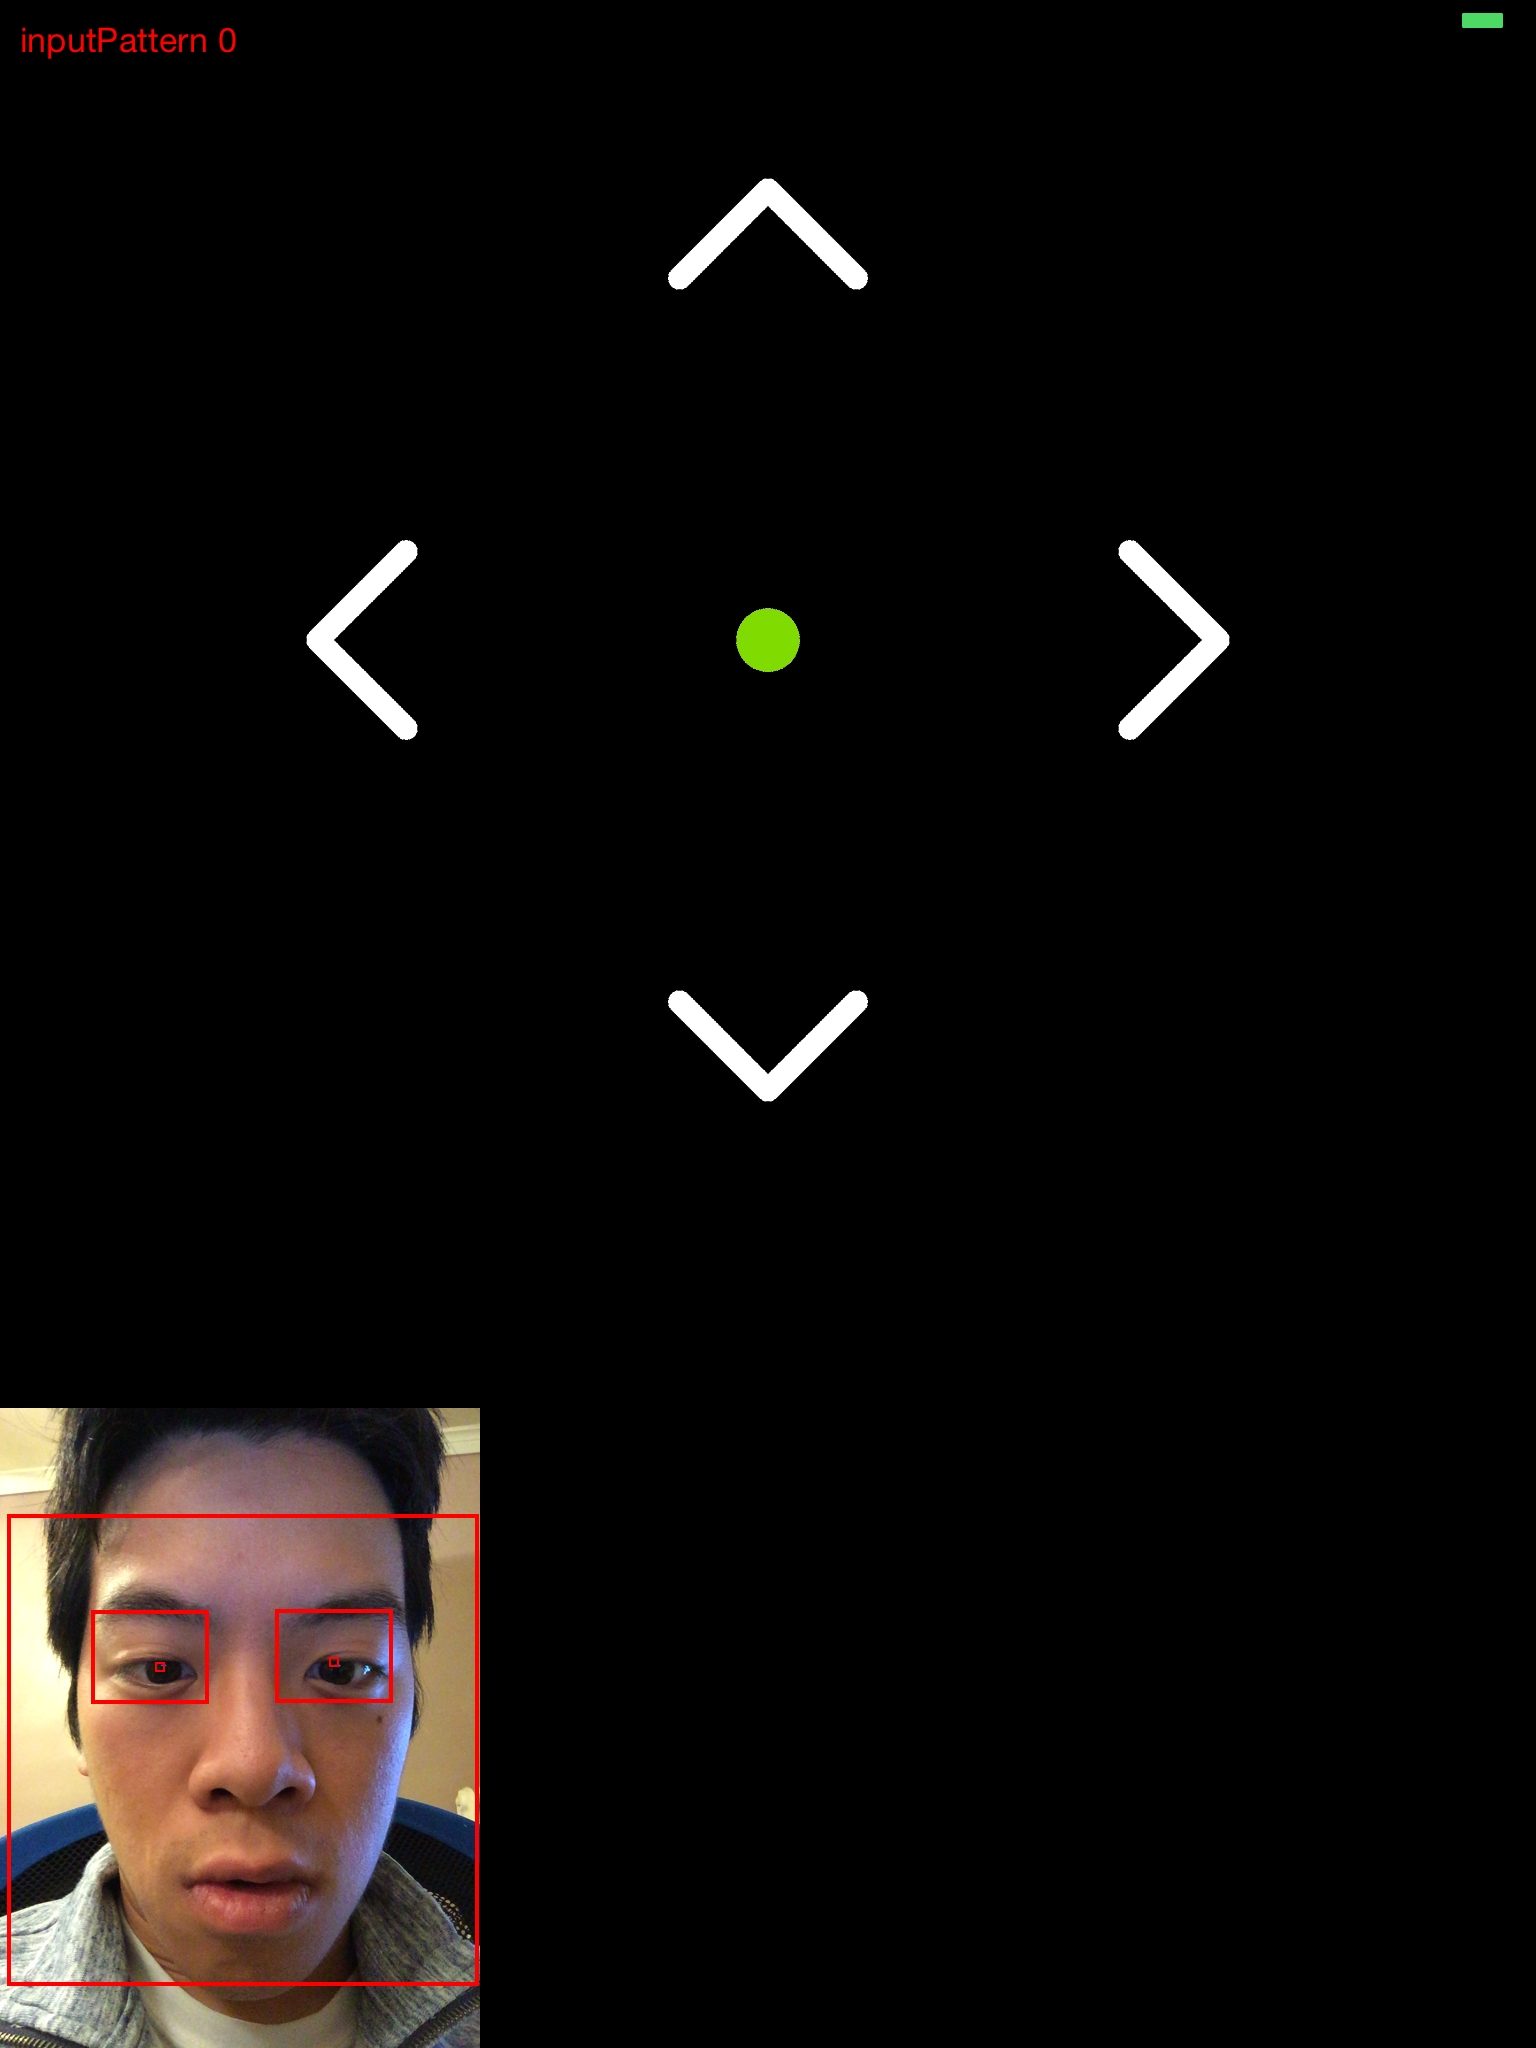
\includegraphics[scale=0.045]{pattern_start}
        \caption{Start calibration}
    \end{subfigure}%
    ~ 
    \begin{subfigure}[t]{0.33\linewidth}
        \centering
        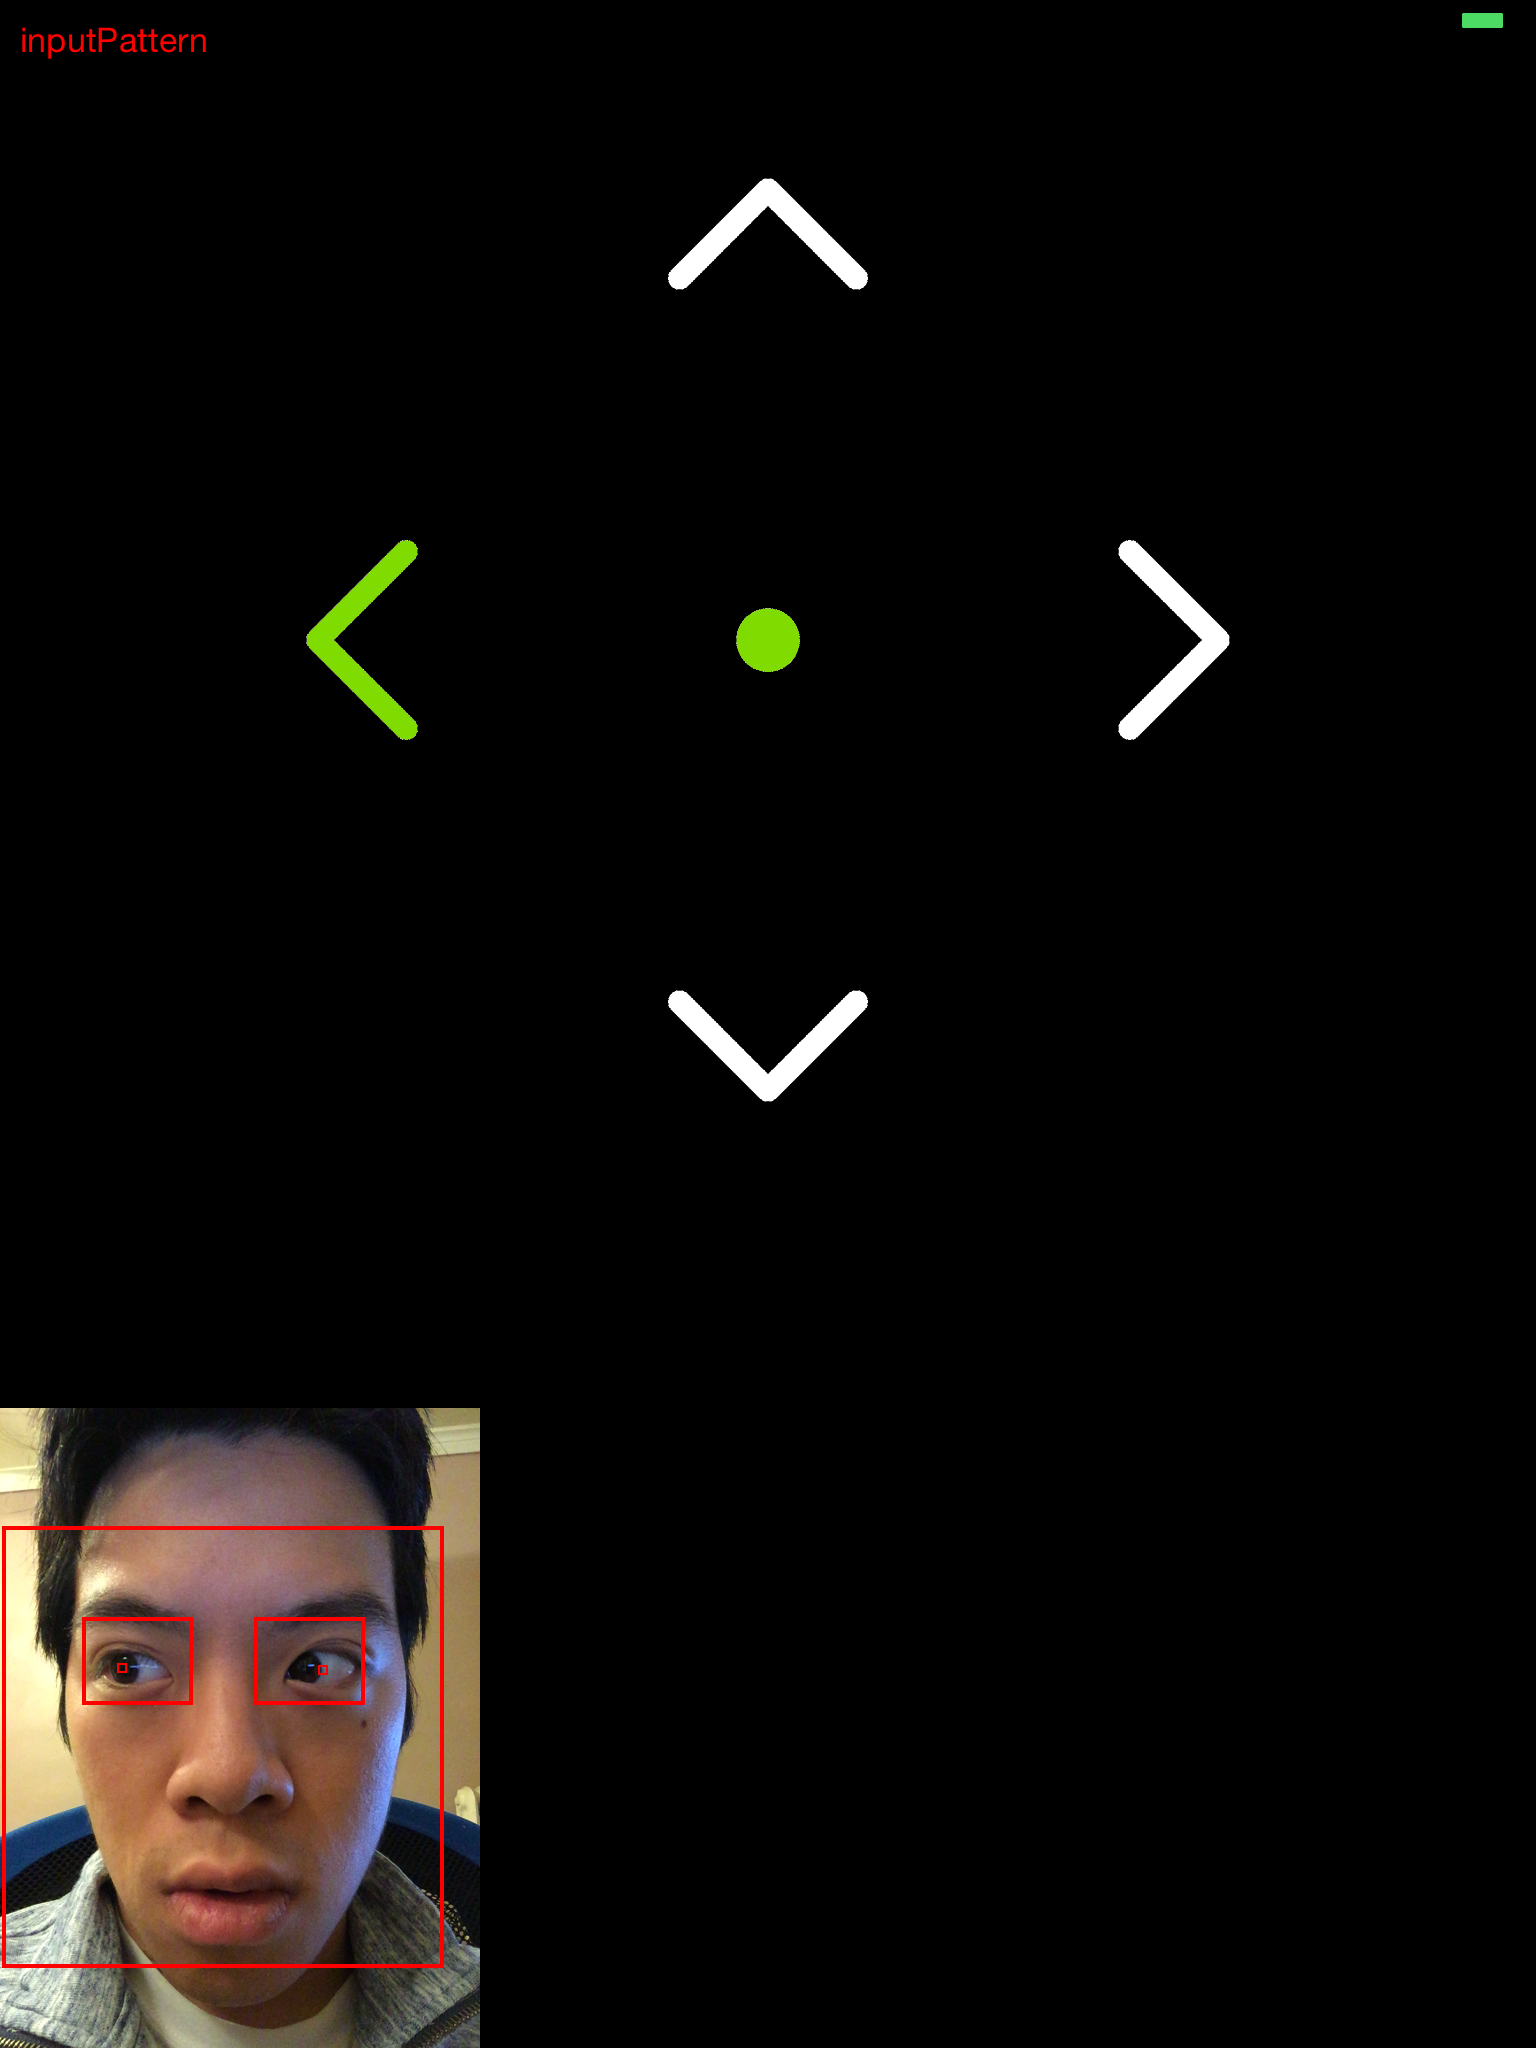
\includegraphics[scale=0.045]{pattern_left}
        \caption{Left gaze}
    \end{subfigure}%
    ~ 
    \begin{subfigure}[t]{0.33\linewidth}
        \centering
        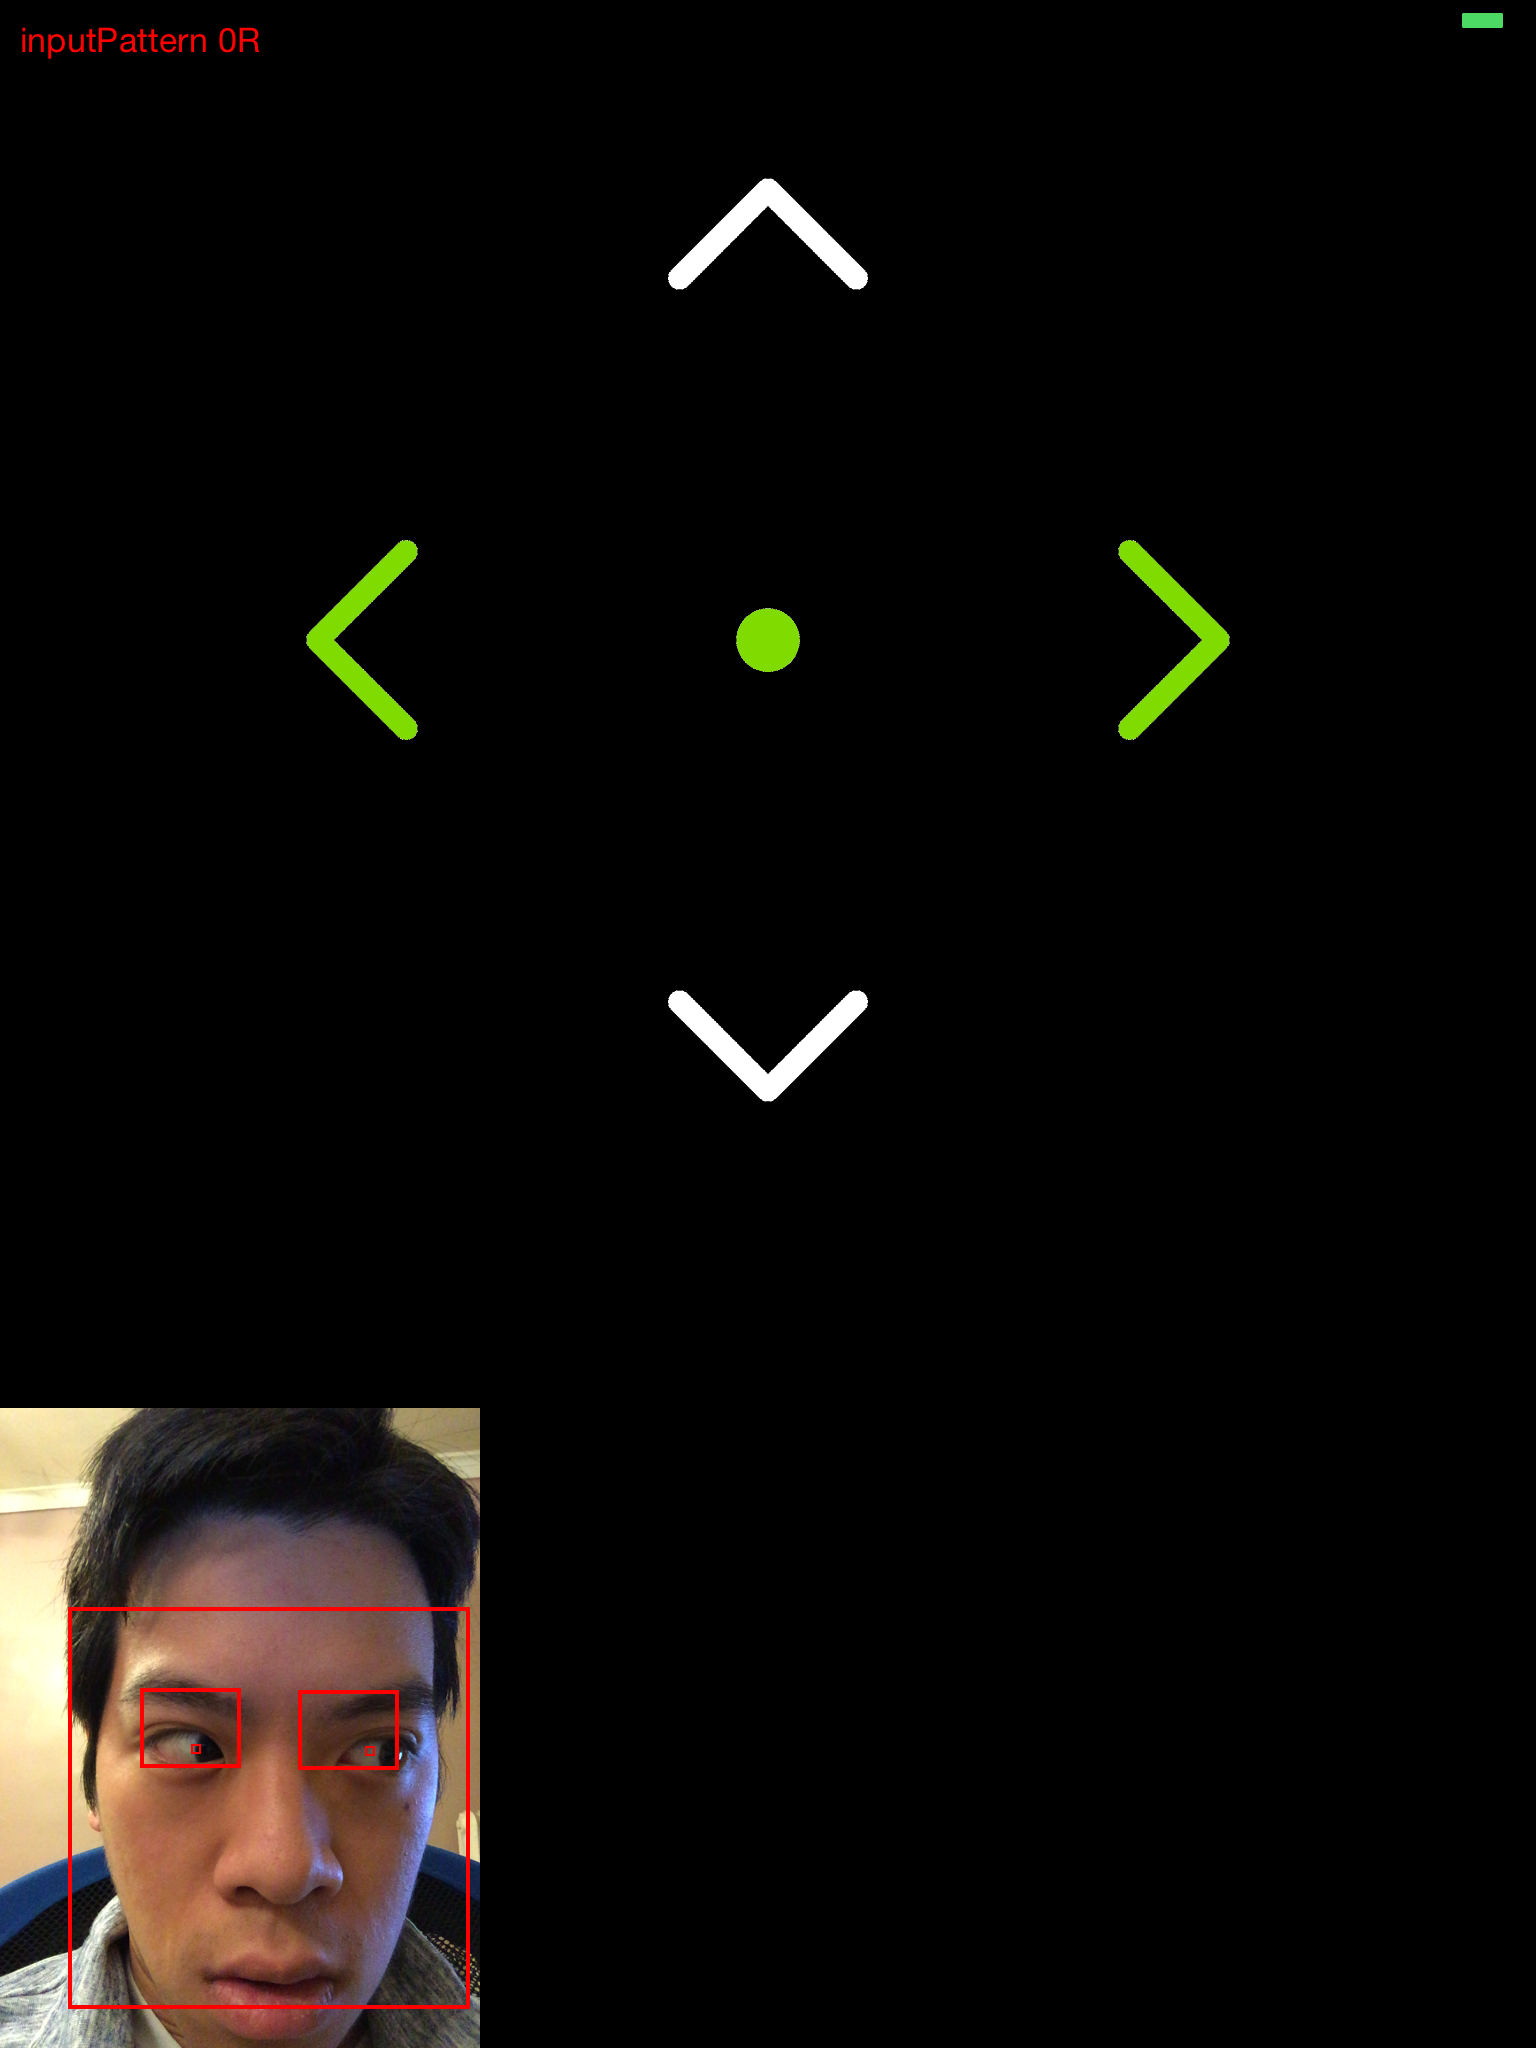
\includegraphics[scale=0.045]{pattern_right}
        \caption{Right gaze}
    \end{subfigure}
    \caption{Pattern unlock sequence}
    \label{pattern}
\end{figure}

\subsection{Performance Optimization Analysis}
Based on the current implementation, an analysis is done on the overall performance.  Given an average frame rate of 35.68 FPS, it is discovered that around 30\% of the computing was directly attributed to the UIImage from CIImage conversion.  It is found that UIImage creation in itself is extremely computationally expensive.  This point can be further asserted from Table \ref{table:houghdraw} that by simply not displaying the small eye patch images in the bottom right corner of the display, the performance can be sped up by 10\% since UIImages are not created for those frames.  In addition, the second highest drainage of processing at 20\% is the CoreImage facial feature detection.  This is expected however, as facial feature detection is nevertheless an expensive operation despite the GPU optimization.

\section{Conclusion}
This implementation demonstrates a successful proof of concept of using gaze estimation approach in mobile security platforms.  It is demonstrated that by only using a monocular camera built in with most mobile devices, it is possible to perform facial feature detection in real-time by optimizing the GPU processes through the CoreImage library.  In addition, by using the relationship between the pupil and the known characteristics with the eye, it is possible to extract the pupil location in such reference frame using various image processing filter techniques.  However, it is noted that since the filters required are inexpensive and the images to be processed are of low resolutions, there is no difference in performance by using OpenCV filters versus GPUImage filters.   Finally, by translating the pupil position across frames, it is then possible to derive the movement and gaze directional changes in the eyes and categorize such movements as distinct directions that can be used as unique keys in a pattern lock sequence. 
\balance
\section{Future Work}
Additional room for improvement can vastly improve on the current implementation.  A useful addition is to develop an inexpensive, GPU-based approach for circle hough transform, thereby allowing the implementation to bypass OpenCV altogether.  Alternatively, exploratory approaches can be done by replacing circle hough transforms with other circle contour detection methods, including binary feature matching, connected pixels, and blob detection.  In addition, instead of using pupil extraction algorithms at each time step, a tracking algorithm like Lucas-Kanade may be explore to track the pupils after a template has been created in the first instance.

Other rooms of improvement in the system implementation includes the use of learning algorithms to determine the parameters for filters used for pupil extraction and facial feature detection.  Finally, by integrating the implementation with a facial recognition algorithm, one can then create a more holistic and practical application in mobile security.

\section{GitHub Page}
The project source code is available at the following address: \url{https://github.com/tamias65/Gaze-Detection-in-iOS-for-Mobile-Application.git}
Since the project checkpoint, the focus has mostly been consistent as planned, but with increasing emphasis on optimization and speed ups of the algorithm rather than exploratory processes of the proof of concept.

{\small
\bibliographystyle{ieee}
\bibliography{egbib}
}

\end{document}
